Испытания представляют собой процесс установления соответствия программы и
программной документации заданным требованиям.

\subsubsection{Проверка требований к документации}
Проверяеться наличие всех документов перечисленных в пyнкте 4.1 данного документа и их соответствие ГОСТ.

\subsection{Проверка требований к интерфейсу}
Интерфейс соответствует схеме, указанной в техническом задании.

\begin{figure}[h!]
    \centering
    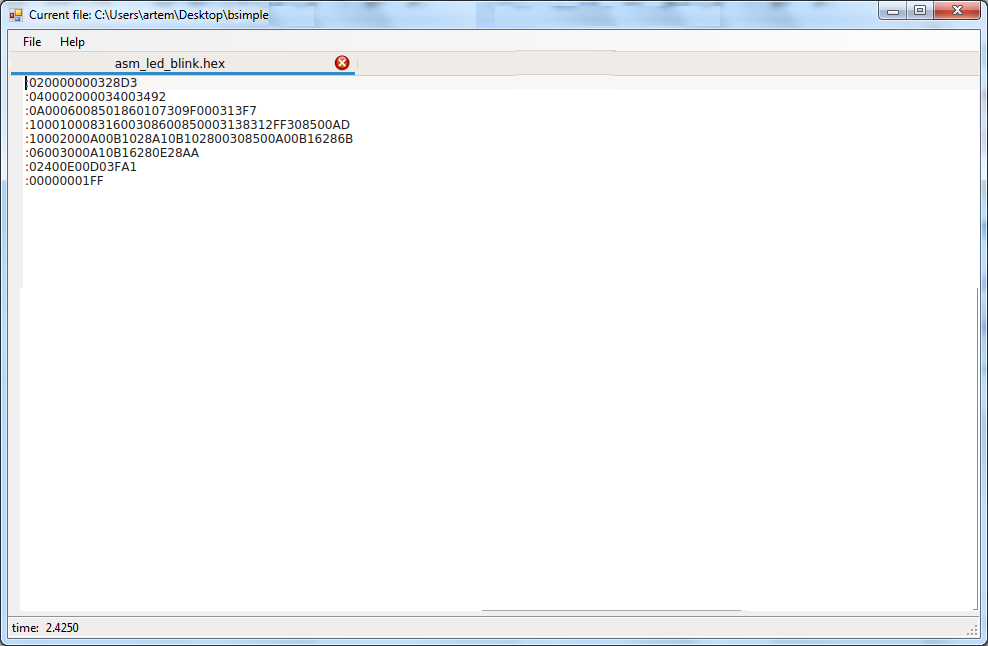
\includegraphics[width=0.5\textwidth]{../screenshots/interface_map.png}
    \caption{Изображение интерфейса программы}
\end{figure}

Интерфейс командной строки также соответствует предъявленным требованиям.

\subsection{Проверка требований к функциональным характеристикам}
Для загрузки данных из формата INTEL HEX8M (.hex) необходимо выбрать его в меню "Open":

\begin{figure}[h!]
    \centering
    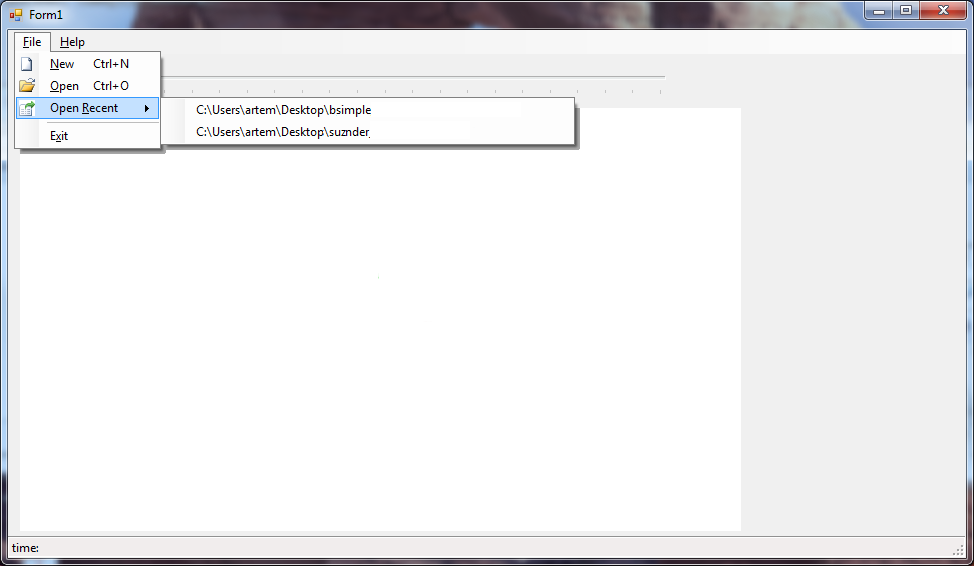
\includegraphics[width=0.8\textwidth]{../screenshots/file_menu_with_recent.png}
    \caption{Загрузка файла}
\end{figure}

Откроется диалог выбора файла:
\begin{figure}[h!]
    \centering
    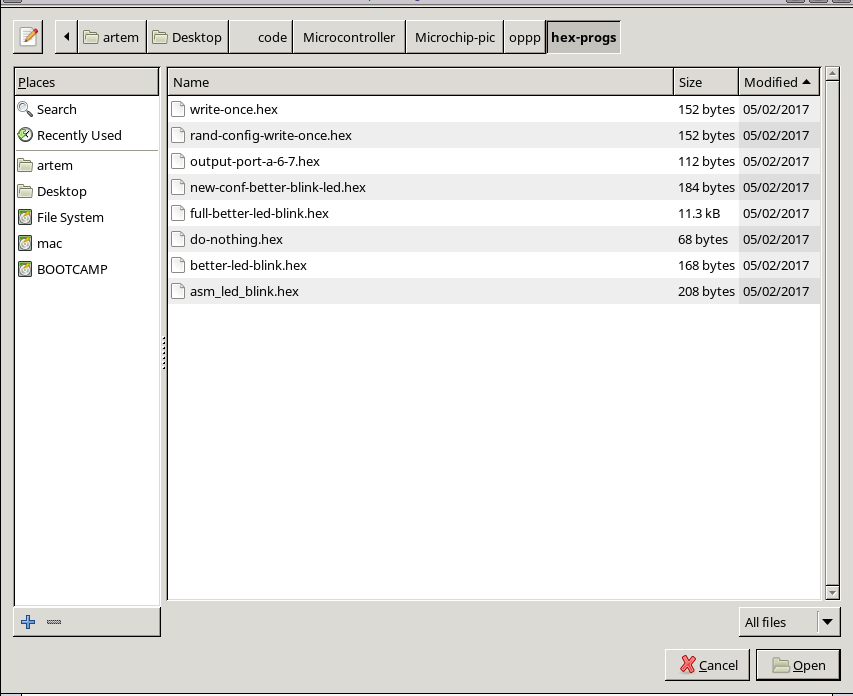
\includegraphics[width=0.5\textwidth]{../screenshots/open_file_dialog.png}
    \caption{Диалог выбора файла}
\end{figure}

После загрузки файла, его содержание будет отображенно в центральном окне.


%=================
Также есть панель для настоек работы программы позволяющая изменять следующие параметры:
\begin{my_enumerate}
\item Указать что требуется запись EEPROM памети без модификации програмной памяти микроконтроллера.
\item Указать что требуется проверить входной файл на ошибки.
\item Указать что требуется записать входной файл в програмную память и в EEPROM память микроконтроллера.
\item Поменять уровень колличества сообщений выводимих программой пользователю.
\item Отменить процесс программирования.
\end{my_enumerate}


%=================
Поддерживатся изменение размеров окна приложения.


\subsection{Проверка требований к надежности}
Оператор должен воспользоваться всеми функциями программы и убедиться, что они не приводят к ее аварийному завершению.
